\documentclass[a4paper,12pt]{article}
\usepackage[utf8x]{inputenc}
\usepackage{amssymb}
\usepackage{amsfonts}
\usepackage{mathrsfs}
\usepackage{amsmath}
\usepackage{amsthm}
\usepackage[margin=3cm]{geometry}
\usepackage{times}
\usepackage{graphicx}
\usepackage{enumitem}
\usepackage{fancyhdr}
\usepackage{hyperref}
\usepackage{setspace}
\usepackage{subcaption}
\usepackage{mathtools}

\usepackage{lineno}
\linenumbers
\renewcommand{\baselinestretch}{1.5}
\usepackage{authblk}

\newtheorem{theorem}{Theorem}
\newtheorem{proposition}{Proposition}[section]
\newtheorem{lemma}{Lemma}[section]
\newtheorem{corollary}{Corollary}[section]
\theoremstyle{definition}
\newtheorem{definition}{Definition}[section]

\newcommand{\boldnabla}{\mbox{\boldmath$\nabla$}} % to be used in mathmode
\newcommand{\cbar}{\overline{\mathbb{C}}}% to be used in mathmode
\newcommand{\diff}[2]{\frac{d #1}{d #2}}% to be used in mathmode
\newcommand{\difff}[2]{\frac{d^2 #1}{d #2^2}}% to be used in mathmode
\newcommand{\pdiff}[2]{\frac{\partial #1}{\partial #2}} % to be used in mathmode
\newcommand{\pdifff}[2]{\frac{\partial^2 #1}{\partial #2^2}}% to be used in mathmode
\newcommand{\upperth}{$^{\mbox{\footnotesize{th}}}$}%to be used in text mode
\newcommand{\vect}[1]{\mathbf{#1}}% to be used in mathmode
\newcommand{\curl}[1]{\boldnabla \times \vect{#1}} % to be used in mathmode
\newcommand{\divr}[1]{\boldnabla \cdot \vect{#1}} %to be used in mathmode
\newcommand{\modu}[1]{\left| #1 \right|} %to be used in mathmode
\newcommand{\brak}[1]{\left( #1 \right)} % to be used in mathmode
\newcommand{\comm}[2]{\left[ #1 , #2 \right]} %to be used in mathmode
\newcommand{\dop}{\vect{d}} %to be used in mathmode
\newcommand{\cov}{\text{cov}} %to be used in mathmode
\newcommand{\var}{\text{var}} %to be used in mathmode
\newcommand{\mb}{\mathbf} %to be used in mathmode
\newcommand{\bs}{\boldsymbol} %to be used in mathmode
% Title Page
\title{A simple two parameter distribution for modelling neuronal activity and capturing neuronal association}
\date{}

\author[1]{Thomas Delaney}
\author[1]{Cian O'Donnell}
\affil[1]{School of Computer Science, Electrical and Electronic Engineering, and Engineering Mathematics, University of Bristol, Bristol, United Kingdom.}
\renewcommand\Affilfont{\itshape\small}

\begin{document}

\maketitle

%\tableofcontents

\abstract{Recent developments in electrophysiological technology have lead to an increase in the size of electrophysiological datasets. Consequently, there is a requirement for new analysis techniques that can make use of these new datasets, while remaining easy to use in practice. In this work, we fit the Conway-Maxwell-binomial distribution to spiking data read from a mouse exposed to visual stimuli.}

\section{Introduction}
  Motivate by pointing out how much computational power it can require to calculate $n$th order correlations.

  Point out that we don't necessarily need to measure correlations anyway.

\section{Results}

  \subsection{Transient increases in mean number of active neurons and variance in number of active neurons at stimulus onset}

  \begin{figure}[h]
    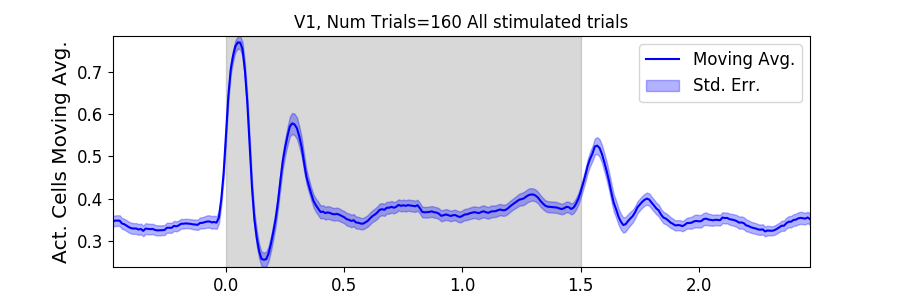
\includegraphics[width=\linewidth]{figures/v1_1ms_moving_avg_all_stimulated_trials.png}
    \caption{A moving average of the number of active neurons in V1. Averages were taken across $100$ms windows split into $100$ bins. The midpoint of the time interval for each window is used as the timepoint (x-axis point) for that window. The shaded area indicates the presence of a visual stimulus. Translucent lines indicate the moving averages for each of the $160$ trials, the opaque line is an average across trials. We can see a transient increase in the average number of active neurons, followed by a fluctuation and another increase.}
    \label{fig:moving_avg_num_active_cells}
  \end{figure}

  \begin{figure}[h]
    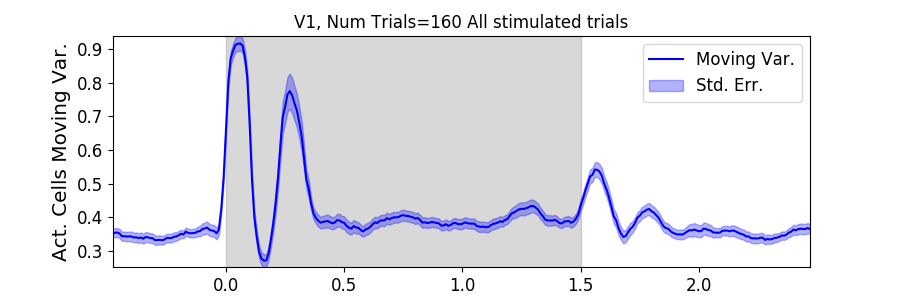
\includegraphics[width=\linewidth]{figures/v1_1ms_moving_var_all_stimulated_trials.png}
    \caption{A moving variance of the number of active neurons in V1. Variances were taken across $100$ms windows split into $100$ bins. The midpoint of the time interval for each window is used as the timepoint (x-axis point) for that window. The shaded area indicates the presence of a visual stimulus. Translucent lines indicate the moving variances for each of the $160$ trials, the opaque line is an average across trials. We can see a transient increase in the variance of the number of active neurons, followed by a fluctuation and another increase.}
    \label{fig:moving_var_num_active_cells}
  \end{figure}

  \subsection{Conway-Maxwell-binomial distribution fits better than binomial or beta-binomial}

  \subsection{Conway-Maxwell-binomial distribution captures changes in association at stimulus onset}

  \subsection{Reproduced stimulus related quenching of neural variability}

\section{Discussion}

\section{Data}
We used data collected by Nick Steinmetz and his lab `CortexLab at UCL' \cite{steinmetz}. The data can be found online \footnote{\url{http://data.cortexlab.net/dualPhase3/}} and are free to use for research purposes.

Two `Phase3' Neuropixels \cite{jun} electrode arrays were inserted into the brain of an awake, head-fixed mouse for about an hour and a half. These electrode arrays recorded $384$ channels of neural data each at $30$kHz and  less than $7$µV RMS noise levels. The sites are densely spaced in a `continuous tetrode'-like arrangement, and a whole array records from a $3.8$mm span of the brain. One array recorded from visual cortex, hippocampus,  and thalamus, the other array recorded from motor cortex and striatum. The data were spike-sorted automatically by Kilosort and manually by N. Steinmetz using Phy. In total 831 well-isolated individual neurons were identified.

  \subsection{Experimental protocol}
  The mouse was shown a visual stimulus on three monitors placed around the mouse at right angles to each other, covering about $\pm 135$ degrees azimuth and $\pm 35$ degrees elevation.

  The stimulus consisted of sine-wave modulated full-field drifting gratings of 16 drift directions ($0^{\circ}, 22.5^{\circ}, \dots, 337.5^{\circ}$) with $2$Hz temporal frequency and $0.08$ cycles/degree spatial frequency displayed for $2$ seconds plus a blank condition. Each of these $17$ conditions were presented $10$ times in a random order across $170$ different trials. There were therefore $160$ trials with a visual stimulus present, and $10$ trials without a visual stimulus.

\section{Methods}
Details about all kinds of things here.
    \subsection{Binning data}
    We converted the spike times for each cell into spike counts by putting the spike times into time bins of a given `width' (in seconds). We used time bins of $1$ms, $5$ms, and $10$ms. We used different time bin widths to assess the impact of choosing a bin width.


    \subsection{Number of \textit{active} neurons}
    To count the number of active neurons in each neuronal ensemble, we split the time interval for each trial into bins of a given width. We counted the number of spikes fired by each cell in each bin. If a cell fired \textit{at least} one spike in a given bin, we regarded that cell as active in that bin. We recorded the number of active cells in every bin, and we recorded each cell's individual spike counts.

    It should be noted that when we used a bin width of $1$ms, the maximum number of spikes in any bin was $1$. For the wider time bins, some bins had spike counts greater than $1$. Consequently when using a bin width of $1$ms, the number of active neurons and the total spike count of a given bin were identical. But for wider bin widths, the total spike count was greater than the number of active neurons.

    So for the $1$ms bin width, the activity of a neuron and the number of spikes fired by that neuron in any bin can be modelled as a Bernoulli variable. But for wider time bins, only the activity can be modelled in this way.

    \subsection{Moving windows for measurements}

    When taking measurements (e.g. moving average over the number of active neurons) or fitting distributions (eg. the beta binomial distribution) we slid a window containing a certain number of bins across the data, and made our measurements at each window position. For example, when analysing $1$ms bin data, we used a window containing $100$ bins, and we slid the window across the time interval for each trial moving $10$ bins at a time. So that for $2560$ms of data, we made $246$ measurements.

    For the $5$ms bin width data, we used windows containing $40$ bins, and slid the window $2$ bins at a time when taking measurements.

    For the $10$ms bin width data, we used windows containing $40$ bins, and slid the window $1$ bin at a time when taking measurements.

    By continuing to use windows containing $40$ bins, we retained statistical power but sacrificed the number of measurements taken.

    There was an interval between each trial with a grey image in place of the moving of the moving bar stimulus. This interval varied in time. But we included some of this interval when recording the data for each trial. We started recording the number of active neurons, and the number of spikes from each neuron from $280$ms before each trial until $280$ms after each trial. This way, we could see the change in our measurements at the onset of a stimulus.

    The actual measurements we took in each window were as follows:
    \begin{description}
      \item[Number of active neurons] The number of neurons firing a spike in each bin. Most of the other measurements are aggregations of these measurements, or models fitted to these measurements.
      \item[Spike counts for each cell] The number of spikes fired by each cell in each bin.
      \item[Moving average] The average number of active cells in each window.
      \item[Moving variance] The variance of the number of active cells in each window.
      \item[Average correlation] We measured the correlation between the spike counts of each pair of cells in the ensemble, and took the average of these measurements.
      \item[Binomial $\mathbf{p}$] We fitted a binomial distribution to the data in each window and recorded the fitted probability of success, $p$ in each case.
      \item[Beta-binomial $\boldsymbol{\alpha}$, $\boldsymbol{\beta}$] We fitted a beta-binomial distribution to the data in each window, and recorded the values of the fitted shape parameters, $\alpha$ and $\beta$, of each distribution.
      \item[Conway-Maxwell-binomial distribution $\mathbf{p}$, $\boldsymbol{\nu}$] We fitted a Conway-Maxwell-binomial distribution to the data in each window, and recorded the fitted values of $p$ and $\nu$ for each distribution.
      \item[Log-likelihoods] We also recorded the log-likelihood of each of the fitted distributions for each window.
    \end{description}

    \subsection{Fano factor}\label{sec:faco_factor}
    The \textit{Fano factor} of a random variable is defined as the ratio of the variable's variance to its mean.
    \begin{align}\label{eq:fano_factor}
      F = \frac{\sigma^2}{\mu}
    \end{align}
    We measured the Fano factor of the spike count of a given cell by measuring the mean and variance of the spike count across trials, and taking the ratio of those two quantities. When calculated in this way the Fano factor can be used as a measure of neural variability.  This is similar to the calculation used in \cite{churchland}.

    \subsection{Probability Distributions suitable for modelling ensemble activity}

    We present here three different probability distributions that could be suitable to model the number of active neurons in an ensemble. Each distribution has the set $\lbrace 0, \dots, n \rbrace$ as its support, where $n$ is the number of neurons in the ensemble. These are simple distributions with either two or three parameters each. However, we regard $n$ as known when using these distributions for modelling, so in effect each distribution has either one or two free parameters.

      \subsubsection{Association}
      \textit{Association} between random variables is similar to the correlation between random variables but is more general in concept. The correlation is a measure of association; and association doesn't have a mathematical definition like correlation does. Essentially, the association between two random variables is their tendency to take the same or similar values. Positively associated variables tend to take the same value, and negatively associated variables tend to take differnt values. In this research, we work with probability distributions of the number of successes in a set of Bernoulli trials. These Bernoulli variables may or may not be associated.

      A probability distribution over the number of successes in $n$ Bernoulli trials, where the Bernoulli variables may be associated, could constitute a good model for the number of active neurons in an ensemble of $n$ neurons.

      \subsubsection{Binomial distribution}
      The binomial distribution is a two parameter discrete probability distribution that can be thought of as a probability distribution the number of successes from $n$ independent Bernoulli trials, each with the same probability of success. The parameters of the binomial distribution are $n$, and $0 \leq p \leq 1$, the probability of success for each of these trials. A random variable with the binomial distribution can take values from $\lbrace 0, \dots, n \rbrace$. The probability mass function of the distribution is
      \begin{align}\label{eq:binomial_pmf}
        P(k;n,p) = \binom{n}{k} p^k (1-p)^{n-k}
      \end{align}

      %%%%%%%%%% MAY REMOVE THIS PART %%%%%%%%%%%%%%
      % If we have $N$ independent samples from a binomial distribution and we know $n$ but want to estimate $p$, we can maximise the log likelihood function
      % \begin{align}\label{eq:binomial_log_like}
      %   L(p) & = \log P(\lbrace k_1, \dots, k_N \rbrace; n,p) \\
      %       & = \sum_{i=1}^N \log \binom{n}{k_i} + k_i \log p + (n-k_i)\log(1-p)
      % \end{align}

      % If we do not know $n$ there is no closed form way way of maximising this equation. Therefore the binomial distribution is generally only used in cases where we do know $n$. Consequently, the distribution is practically a one parameter distribution.
      %%%%%%%%%%%%%%%%%%%%%%%%%%%%%%%%%%%%%%%%%%%%%%

      As model for the activity of a neuronal ensemble, the main problem with the binomial distribution is that it treats each neuron, represented as a Bernoulli trial, as independent. It is well know that neurons are not independent, and that correlated behaviour between neurons is vital for representing sensory information. The binomial distribution falls short in this regard, but it is useful as performance benchmark when assessing the performance of other models.

      \subsubsection{Beta-binomial distribution}
      The beta distribution is the conjugate distribution of the binomial distribution. The beta-binomial distribution is the combination of the beta distribution and the binomial distribution, in that the probability of success for the binomial distribution is sampled from the beta distribution. This allows the beta-binomial distribution to capture some over dispersion relative to the binomial distribution.

      The beta-binomial distribution is a three parameter distribution, $n$ the number of Bernoulli trials, and $\alpha \in \mathbb{R}_{>0}$ and $\beta \in \mathbb{R}_{>0}$ the shape parameters of the beta distribution. The probability mass function for the beta-binomial distribution is
      \begin{align}\label{eq:betabinomial_pdf}
        P(k;n, \alpha, \beta) = \binom{n}{k}\frac{B(k + \alpha, n - k + \beta)}{B(\alpha, \beta)}
      \end{align}
      where $B(\alpha, \beta)$ is the beta function.

      This probability distribution can be reparametrised in a number of ways. One of which defines new parameters $\pi$ and $\rho$ by
      \begin{align}\label{eq:betabinomial_reparam}
        \pi &= \frac{\alpha}{\alpha + \beta} \\
        \rho &= \frac{1}{\alpha + \beta + 1}
      \end{align}
      This reparametrisation is useful because $\pi$ acts as a location parameter analogous to the $p$ parameter of a binomial distribution. A value of $\rho > 0$ indicates over-dispersion relative to a binomial distribution.

      As a model for the activity of a neuronal ensemble, the beta-binomial distribution is more suitable than a binomial distribution because the over-dispersion of the beta-binomial distribution can be used to model positive association between the neurons. An extreme example of this over-dispersion/positive association can be seen in figure \ref{fig:betabinomial_big_overdispersion}. In this figure, the neurons are positively associated and so tend to take the same value, consequently the probability mass of the beta-binomial distribution builds up close to $k=0$ and $k=n$. It is worth noting that the location parameter for each distribution has the same value, $p=\pi=0.5$.

      \begin{figure}[h]
        \begin{subfigure}[h]{0.5\linewidth}
          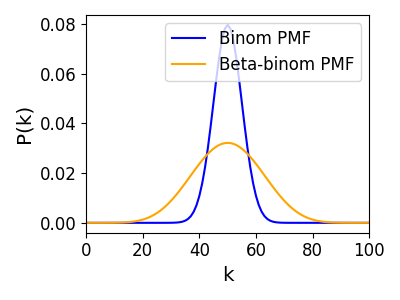
\includegraphics[width=\textwidth]{figures/betabinomial_overdispersion.png}
          \caption{$n=100, p=0.5, \alpha=\beta=10$}
          \label{fig:betabinomial_overdispersion}
        \end{subfigure}
        \begin{subfigure}[h]{0.5\linewidth}
          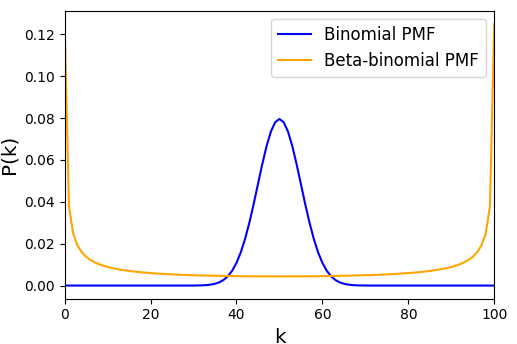
\includegraphics[width=\textwidth]{figures/betabinomial_big_overdispersion.png}
          \caption{$n=100, p=0.5, \alpha=\beta=0.3$}
          \label{fig:betabinomial_big_overdispersion}
        \end{subfigure}
        \caption{Figures showing the over-dispersion possible for a beta-binomial distribution relative to a binomial distribution. Parameters are shown in the captions. }
      \end{figure}

      \subsubsection{Conway-Maxwell-binomial distribution}
      The Conway-Maxwell-binomial distribution (COMb distribution) is a three parameter generalisation of the binomial distribution that allows for over dispersion and under dispersion relative to the binomial distribution. The parameters of the distribution are $n$ the number of Bernoulli trials, $0 \leq p \leq 1$, the location parameter, and $\nu \in \mathbb{R}$ the shape parameter.

      The probability mass function of the COMb distribution is
      \begin{align}\label{eq:comb_pmf}
        P(k;n,p,\nu) = \frac{1}{S(n,p,\nu)}\binom{n}{k}^{\nu} p^k (1-p)^{n-k}
      \end{align}
      where
      \begin{align}\label{eq:comb_norm}
        S(n,p,\nu) = \sum_{j=0}^n \binom{n}{k}^{\nu} p^j (1-p)^{n-j}
      \end{align}
      The only difference between this PMF and the PMF for the standard binomial is the introduction of $\nu$ and the consequent introduction of the normalising function $S(n,p,\nu)$.

      Indeed, if $\nu = 1$ the COMb distribution is identical to the binomial distribution with the same values for $n$ and $p$. We can see in figure \ref{fig:comb_bin_dkl} that the KL-divergence $D_{KL}(P_{COMb}(n,p,\nu), P_{Bin}(n,p))=0$ along the line where $\nu=1$.

      If $\nu < 1$ the COMb distribution will exhibit over-dispersion relative to the binomial distribution. If $p=0.5$ and $\nu=0$ the COMb distribution is the discrete uniform distribution, and if $\nu < 0$ the mass of the COMb distribution will tend to build up near $k=0$ and $k=n$. This over-dispersion represents positive association in the Bernoulli variables. An example of this over-dispersion can be seen in figure \ref{fig:comb_overrdispersion}.

      If $\nu > 1$ the COMb distribution will exhibit under-dispersion relative to the binomial distribution. The larger the value of $\nu$ the more probability mass will build up at $n/2$ for even $n$, or at $\lfloor n/2 \rfloor$ and $\lceil n/2 \rceil$ for odd $n$. This under-dispersion represents negative association in the Bernoulli variables. An example of this under-dispersion can be seen in figure \ref{fig:comb_underdispersion}.

      It should be noted that the shape parameter of the COMb distribution, $p$, does not correspond to the mean of the distribution, as is the case for the binomial and beta-binomial distributions. An illustration of this can be seen in figure \ref{fig:comb_skewed}. This is because an interaction between the $p$ and $\nu$ parameters skews the mean. There is no analytical expression for the mean of the COMb distribution.

      \begin{center}
        \begin{tabular}[h]{|c|c|c|}
          \hline
          $\boldsymbol{\nu}$  & \textbf{Relative dispersion}  & \textbf{Associaton between neurons/variables} \\ \hline
          $<1$                & over                          & positive                                      \\ \hline
          $0$                 & none                          & none                                          \\ \hline
          $>1$                & under                         & negative                                      \\ \hline
        \end{tabular}
      \end{center}

      Since the COMb distribution has the potential to capture positive and negative associatons between the neurons/Bernoulli variables, it should be an excellent candidate for modelling the number of active neurons in a neuronal ensemble.

      We wrote a dedicated Python package to enable easy creation and fitting of COMb distribution objects. The format of the package imitates the format of other distribution objects from the \texttt{scipy.stats} Python package. The COMb package can be found here: \\
      \url{https://github.com/thomasjdelaney/Conway_Maxwell_Binomial_Distribution}

      \newpage

      \begin{figure}[h]
        \begin{subfigure}[h]{0.5\linewidth}
          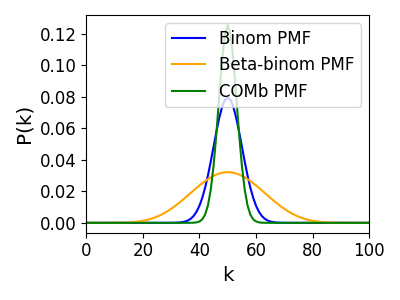
\includegraphics[width=\textwidth]{figures/comb_underdispersion.png}
          \caption{$n=100, p=0.5, \alpha=\beta=10, \nu=2.5$}
          \label{fig:comb_underdispersion}
        \end{subfigure}
        \begin{subfigure}[h]{0.5\linewidth}
          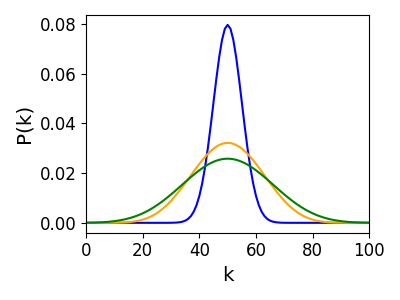
\includegraphics[width=\textwidth]{figures/comb_overrdispersion.png}
          \caption{$n=100, p=0.5, \alpha=\beta=0.3, \nu=0.1$}
          \label{fig:comb_overrdispersion}
        \end{subfigure}
        \begin{subfigure}[h]{0.5\linewidth}
          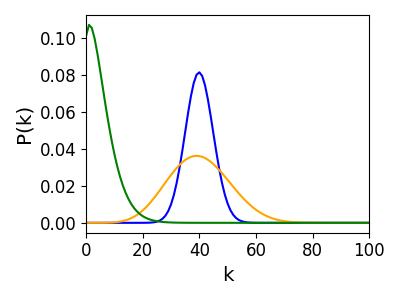
\includegraphics[width=\textwidth]{figures/comb_skewed.png}
          \caption{$n=100, p=0.4, \alpha=10, \beta=15, \nu=0.1$}
          \label{fig:comb_skewed}
        \end{subfigure}
        \begin{subfigure}[h]{0.5\linewidth}
          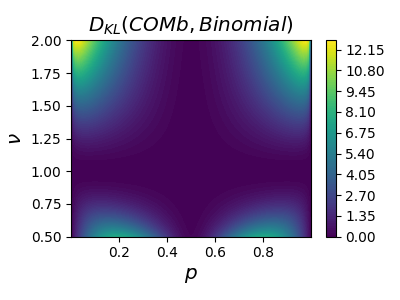
\includegraphics[width=\textwidth]{figures/comb_bin_dkl.png}
          \caption{KL-Divergence as a function of $p$ and $\nu$. $n=100$.}
          \label{fig:comb_bin_dkl}
        \end{subfigure}
        \caption{Figures showing (a) the over-dispersion and (b) under-dispersion permitted by the COMb distribution. (c) illustrates that the shape parameter of the COMb distribution, $p$, does not correspond to the mean of the distribution, as it does for the binomial and beta-binomial distributions. (d) shows a heatmap for the value of the Kullback-Liebler divergence between the COMb distribution and the standard binomial distribution with same value for $n$, as a function of $p$ and $\nu$. Parameters are shown in the captions.}
      \end{figure}

      \newpage

    \subsection{Fitting}
    We fitted a binomial, beta-binomial, and Conway-Maxwell-binomial (COMb) distribution to the neural activity in each of the overlapping windows covering each trial. To fit the distributions we minimised the appropriate negative log likelihood function using the data from the window.

    There is an analytical solution for the binomial distribution.
    \begin{align}\label{eq:binomial_log_like_p_estimate}
      \hat{p} = \frac{1}{n}\sum_{i=1}^N k_i
    \end{align}

    We minimised the negative log likelihood function of the beta-binomial distribution numerically.

    The log likelihood function of the COMb distribution is
    \begin{align}\label{eq:comb_log_like}
      \ell (p,\nu | k_1,\dots,k_N) =& N\left[n\log(1-p) - \log S(n,p,\nu)\right]  \\
        &+ \log \frac{p}{1-p} \sum_{i=1}^N k_i \\
        &+ \nu \sum_{i=1}^N \log \binom{n}{k_i}
    \end{align}
    We minimised the negation of this function using numerical methods.

    More specifically, we used the \texttt{minimise} function of the \texttt{scipy.optimize} Python package.

    \subsection{Goodness-of-fit}
    After fitting, we measured the goodness-of-fit of each model/distribution with their log likelihood. We calculated this directly using the \texttt{logpmf} functions of the distribution objects in Python.

\section{Discussion}
Point out that the Conway-Maxwell-binomial distribution could be used to measure activity and association without having to sort the voltage traces into spikes. That does defeat the purpose slightly, however.

\newpage
\bibliography{conway_maxwell_hierarchical_model.bbl}

\end{document}
